\documentclass[twoside]{book}

% Packages required by doxygen
\usepackage{calc}
\usepackage{doxygen}
\usepackage{graphicx}
\usepackage[utf8]{inputenc}
\usepackage{makeidx}
\usepackage{multicol}
\usepackage{multirow}
\usepackage{textcomp}
\usepackage[table]{xcolor}

% Font selection
\usepackage[T1]{fontenc}
\usepackage{mathptmx}
\usepackage[scaled=.90]{helvet}
\usepackage{courier}
\usepackage{amssymb}
\usepackage{sectsty}
\renewcommand{\familydefault}{\sfdefault}
\allsectionsfont{%
  \fontseries{bc}\selectfont%
  \color{darkgray}%
}
\renewcommand{\DoxyLabelFont}{%
  \fontseries{bc}\selectfont%
  \color{darkgray}%
}

% Page & text layout
\usepackage{geometry}
\geometry{%
  a4paper,%
  top=2.5cm,%
  bottom=2.5cm,%
  left=2.5cm,%
  right=2.5cm%
}
\tolerance=750
\hfuzz=15pt
\hbadness=750
\setlength{\emergencystretch}{15pt}
\setlength{\parindent}{0cm}
\setlength{\parskip}{0.2cm}
\makeatletter
\renewcommand{\paragraph}{%
  \@startsection{paragraph}{4}{0ex}{-1.0ex}{1.0ex}{%
    \normalfont\normalsize\bfseries\SS@parafont%
  }%
}
\renewcommand{\subparagraph}{%
  \@startsection{subparagraph}{5}{0ex}{-1.0ex}{1.0ex}{%
    \normalfont\normalsize\bfseries\SS@subparafont%
  }%
}
\makeatother

% Headers & footers
\usepackage{fancyhdr}
\pagestyle{fancyplain}
\fancyhead[LE]{\fancyplain{}{\bfseries\thepage}}
\fancyhead[CE]{\fancyplain{}{}}
\fancyhead[RE]{\fancyplain{}{\bfseries\leftmark}}
\fancyhead[LO]{\fancyplain{}{\bfseries\rightmark}}
\fancyhead[CO]{\fancyplain{}{}}
\fancyhead[RO]{\fancyplain{}{\bfseries\thepage}}
\fancyfoot[LE]{\fancyplain{}{}}
\fancyfoot[CE]{\fancyplain{}{}}
\fancyfoot[RE]{\fancyplain{}{\bfseries\scriptsize Generated on Wed Jul 17 2019 16\-:16\-:40 for My Project by Doxygen }}
\fancyfoot[LO]{\fancyplain{}{\bfseries\scriptsize Generated on Wed Jul 17 2019 16\-:16\-:40 for My Project by Doxygen }}
\fancyfoot[CO]{\fancyplain{}{}}
\fancyfoot[RO]{\fancyplain{}{}}
\renewcommand{\footrulewidth}{0.4pt}
\renewcommand{\chaptermark}[1]{%
  \markboth{#1}{}%
}
\renewcommand{\sectionmark}[1]{%
  \markright{\thesection\ #1}%
}

% Indices & bibliography
\usepackage{natbib}
\usepackage[titles]{tocloft}
\setcounter{tocdepth}{3}
\setcounter{secnumdepth}{5}
\makeindex

% Hyperlinks (required, but should be loaded last)
\usepackage{ifpdf}
\ifpdf
  \usepackage[pdftex,pagebackref=true]{hyperref}
\else
  \usepackage[ps2pdf,pagebackref=true]{hyperref}
\fi
\hypersetup{%
  colorlinks=true,%
  linkcolor=blue,%
  citecolor=blue,%
  unicode%
}

% Custom commands
\newcommand{\clearemptydoublepage}{%
  \newpage{\pagestyle{empty}\cleardoublepage}%
}


%===== C O N T E N T S =====

\begin{document}

% Titlepage & ToC
\hypersetup{pageanchor=false}
\pagenumbering{roman}
\begin{titlepage}
\vspace*{7cm}
\begin{center}%
{\Large My Project }\\
\vspace*{1cm}
{\large Generated by Doxygen 1.8.5}\\
\vspace*{0.5cm}
{\small Wed Jul 17 2019 16:16:40}\\
\end{center}
\end{titlepage}
\clearemptydoublepage
\tableofcontents
\clearemptydoublepage
\pagenumbering{arabic}
\hypersetup{pageanchor=true}

%--- Begin generated contents ---
\chapter{Code Structure}
\label{codestructure}
\hypertarget{codestructure}{}
The code is divided into three parts\-: the (optional) parameters file, user defined functions, and core functions. The parameters file includes the definition of parameters used in the simulation (mesh refinement, time step size, material parameters, etc.). The user defined functions is a list of functions that can/must be defined by the user. The {\ttfamily define\-Parameters} and {\ttfamily residual} functions (italicized) require a user definition; the remaining functions have default definitions that can be overridden by the user if desired. These user functions are called by the core functions, as shown in the following diagram.

\begin{center}

\begin{DoxyImageNoCaption}
  \mbox{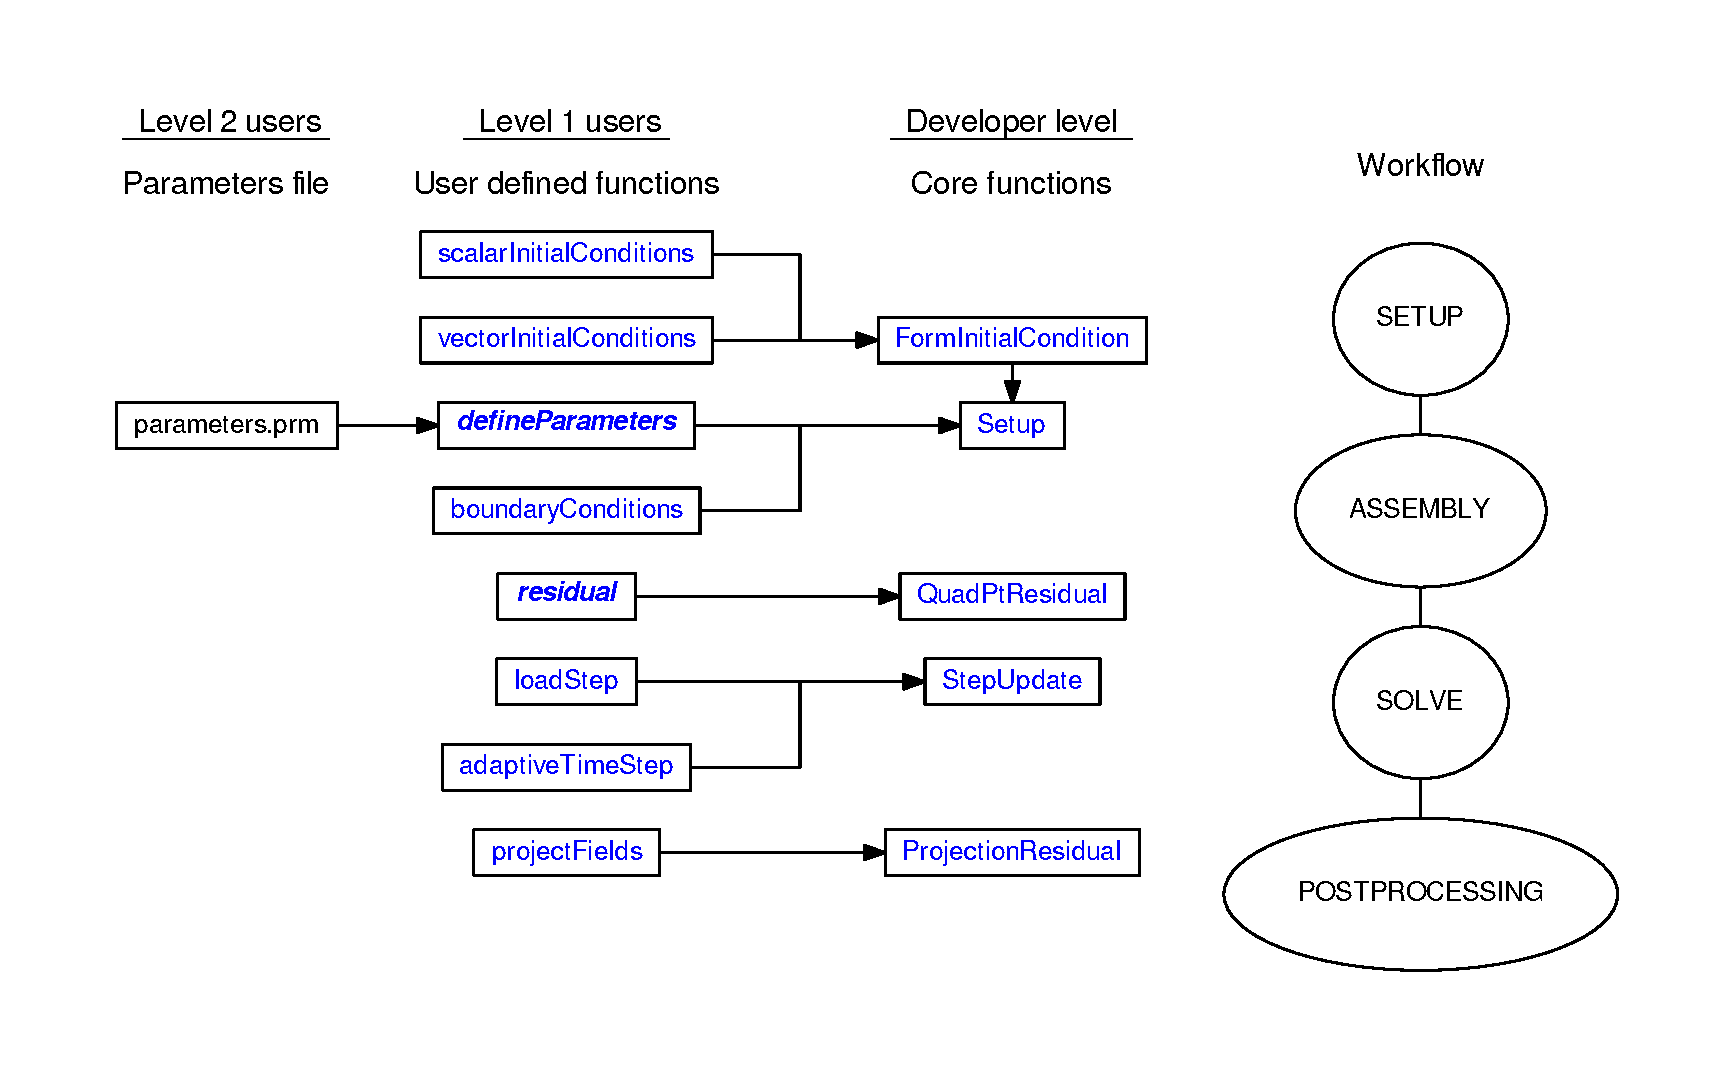
\includegraphics[width=\textwidth,height=\textheight/2,keepaspectratio=true]{dot_inline_dotgraph_1}}
\end{DoxyImageNoCaption}
\end{center}
 
\chapter{Example 1 \-: Nongradient, finite strain elasticity}
\label{example1}
\hypertarget{example1}{}


This example implements static finite strain elasticity in 3\-D, with a combination of Dirichlet and Neumann boundary conditions. We solve for the displacement vector field, with the following weak form\-:

\begin{eqnarray*} \int_\Omega (\nabla{\boldsymbol{w}}:\boldsymbol{P}) dV - \int_{\partial\Omega} (\boldsymbol{w}\cdot\boldsymbol{h}) dS = 0 \end{eqnarray*}

With the loading specified in the below code, the following deformation occurs\-:

 

\section*{Implementation\-: Level 1 users }

To model nongradient, finite strain elasticity, we will specify the following through defining user functions\-: \par

\begin{DoxyItemize}
\item Boundary conditions \par

\item Derived fields for output (e.\-g. eqivalent stress) \par

\item Constitutive model (via the 1st Piola-\/\-Kirchhoff stress) \par

\item Parameter values \par

\item Weak form of the P\-D\-E \par

\end{DoxyItemize}

First, we include the header file declaring the required user functions. These functions will be defined in this file.


\begin{DoxyCodeInclude}

\end{DoxyCodeInclude}


Now, we first define any optional user functions. Optional user functions have a default definition that can be redefined by the user using a function pointer. This will be done in the {\ttfamily define\-Parameters} function. The available list of optional user functions includes\-: {\ttfamily boundary\-Conditions}, {\ttfamily scalar\-Initial\-Conditions}, {\ttfamily vector\-Initial\-Conditions}, {\ttfamily load\-Step}, {\ttfamily adaptive\-Time\-Step}, and {\ttfamily project\-Fields}. In this example, we redefine the {\ttfamily boundary\-Conditions} and {\ttfamily project\-Fields} functions, while using the default functions for the others.

{\bfseries  The {\ttfamily boundary\-Conditions} function }

This function defines Dirichlet boundary conditions using Pet\-I\-G\-A's {\ttfamily I\-G\-A\-Set\-Boundary\-Value} function. The arguments to this function are as follows\-: the iga object (user.\-iga), the \char`\"{}axis\char`\"{} (0, 1, or 2, corresponding to the x, y, or z-\/axis), the \char`\"{}side\char`\"{} (0 or 1), the \char`\"{}dof\char`\"{}, and the \char`\"{}value\char`\"{} that is to be imposed. Note that this can only set a uniform value for a degree-\/of-\/freedom on any side. Here, we fix all three degrees-\/of-\/freedom on the surface at z=0.


\begin{DoxyCodeInclude}

\end{DoxyCodeInclude}


{\bfseries  The {\ttfamily project\-Fields} function }

If there are field values derived from the solution fields that are of interest, we can compute these values at each quadrature point and project the value to the nodes. Here, we compute the equivalent stress using the 1st Piola-\/\-Kirchhoff stress. Scalar values are stored in the {\ttfamily scalar\-Projections} vector and vector values are stored in the {\ttfamily vector\-Projections} vector.


\begin{DoxyCodeInclude}

\end{DoxyCodeInclude}


{\bfseries  The {\ttfamily get1st\-Piola\-Kirchhoff} function }

This function defines the 1st Piola-\/\-Kirchhoff stress. However, it is used only in this file (by the {\ttfamily project\-Fields} and {\ttfamily residual} functions), so it is not a class member function nor does it have an associated function pointer. Additional nonmember functions can be defined in this file, if they are only used by other functions in this same file.


\begin{DoxyCodeInclude}

\end{DoxyCodeInclude}


{\bfseries  The {\ttfamily define\-Parameters} function }

The user is required to define the {\ttfamily define\-Parameters} and {\ttfamily residual} functions. The {\ttfamily define\-Parameters} defines variables and functions in the {\ttfamily App\-Ctx} object. The {\ttfamily App\-Ctx} object is defined in the app\-Ctx.\-h file. This function is used to define any values in {\ttfamily user} that will be needed in the problem. It is also used to set any function pointers for user functions that we have redefined.


\begin{DoxyCodeInclude}

\end{DoxyCodeInclude}


Here, we define the mesh by setting the number of elements in each direction, e.\-g. a 10x10x10 element mesh.


\begin{DoxyCodeInclude}

\end{DoxyCodeInclude}


We also define the dimensions of the domain, e.\-g. a unit cube.


\begin{DoxyCodeInclude}

\end{DoxyCodeInclude}


We specify the number of vector and scalar solution and projection fields by adding the name of each field to their respective vector. Here, we have one vector solution field (the displacement) and one scalar projection field (the von Mises stress). We do not use any scalar solution or vector projection fields in this example.


\begin{DoxyCodeInclude}

\end{DoxyCodeInclude}


We can specify the polynomial order of the basis splines, as well as the global continuity. Note that the global continuity must be less than the polynomial order. Here, we use a linear basis function with C-\/0 continuity.


\begin{DoxyCodeInclude}

\end{DoxyCodeInclude}


We now define the 4th order elasticity tensor. Note that we use the C++ map {\ttfamily user.\-mat\-Param} whenever we'd like to be able to define the parameter value in the parameters file (see the end of this page).


\begin{DoxyCodeInclude}

\end{DoxyCodeInclude}


We specify a scalar coefficient to the Neumann boundary condition.


\begin{DoxyCodeInclude}

\end{DoxyCodeInclude}


Finally, we redirect the desired user function pointers to the {\ttfamily boundary\-Conditions} and {\ttfamily project\-Fields} functions that we defined above. This completes the {\ttfamily define\-Parameters} function.


\begin{DoxyCodeInclude}

\end{DoxyCodeInclude}


{\bfseries  The {\ttfamily residual} function }

The residual function defines the residual that is to be driven to zero. This is the central function of the code. It is set up to follow the analytical weak form of the P\-D\-E. It has a number of arguments that give problem information at the current quadrature point.


\begin{DoxyCodeInclude}

\end{DoxyCodeInclude}


{\ttfamily d\-V} is a boolean, \char`\"{}true\char`\"{} if {\ttfamily residual} is being called for the volume integral and \char`\"{}false\char`\"{} if {\ttfamily residual} is being called for the surface integral.\par
{\ttfamily d\-S} is a boolean, \char`\"{}false\char`\"{} if {\ttfamily residual} is being called for the volume integral and \char`\"{}true\char`\"{} if {\ttfamily residual} is being called for the surface integral.\par
{\ttfamily x} gives the coordinates of the quadrature point.\par
{\ttfamily normal} gives the unit normal for a surface quadrature point.\par
{\ttfamily c} gives the information (values, gradients, etc.) for the scalar solution fields at the current quadrature point (see documentation for solution\-Scalars class).\par
{\ttfamily u} gives the information (values, gradients, etc.) for the vector solution fields at the current quadrature point (see documentation for solution\-Vectors class).\par
{\ttfamily w1} gives the information for the scalar test functions.\par
{\ttfamily w2} gives the information for the vector test functions.\par
{\ttfamily user} is a structure available for parameters related to the initial boundary value problem (e.\-g. elasticity tensor).\par
{\ttfamily r} stores the scalar value of the residual for the weak form of the P\-D\-E which is then used by the core assembly functions.

The following functions are available for the solution objects {\ttfamily c} and {\ttfamily u}, where the argument is the field index, i.

{\ttfamily c.\-val(i)} -\/ Value of scalar field i, scalar \par
{\ttfamily c.\-grad(i)} -\/ Gradient of scalar field i, 1st order tensor \par
{\ttfamily c.\-hess(i)} -\/ Hessian of scalar field i, 2nd order tensor \par
{\ttfamily c.\-laplacian(i)} -\/ Laplacian of scalar field i, scalar \par
{\ttfamily c.\-val\-P(i)} -\/ Value of scalar field i at previous time step, scalar \par
{\ttfamily c.\-grad\-P(i)} -\/ Gradient of scalar field i at previous time step, 1st order tensor \par
{\ttfamily c.\-hess\-P(i)} -\/ Hessian of scalar field i at previous time step, 2nd order tensor \par
{\ttfamily c.\-laplacian\-P(i)} -\/ Laplacian of scalar field i at previous time step, scalar

{\ttfamily u.\-val(i)} -\/ Value of vector field i, 1st order tensor \par
{\ttfamily u.\-grad(i)} -\/ Gradient of vector field i, 2nd order tensor \par
{\ttfamily u.\-hess(i)} -\/ Hessian of vector field i, 3rd order tensor \par
{\ttfamily u.\-val\-P(i)} -\/ Value of vector field i at previous time step, 1st order tensor \par
{\ttfamily u.\-grad\-P(i)} -\/ Gradient of vector field i at previous time step, 2nd order tensor \par
{\ttfamily u.\-hess\-P(i)} -\/ Hessian of vector field i at previous time step, 3rd order tensor

Similar functions are available for the test functions. Also, the following tensor operations are useful\-:

Tensor operations\-: \par
{\ttfamily operator+} -\/ tensor addition \par
{\ttfamily operator-\/} -\/ tensor subraction \par
{\ttfamily operator$\ast$} -\/ single contraction between tensors or scalar multiplication \par
{\ttfamily double\-\_\-contract} -\/ double contraction of two 2nd order tensors, or a 4th order tensor and a 2nd order tensor. \par
{\ttfamily trans( )} -\/ transpose 2nd order tensor \par
{\ttfamily trace( )} -\/ trace of 2nd order tensor \par
{\ttfamily det( )} -\/ determinant of 2nd order tensor \par
{\ttfamily inv( )} -\/ inverse of 2nd order tensor \par


The example code here implements the weak form for finite strain elasticity, $\int_\Omega (\nabla{\boldsymbol{w}}:\boldsymbol{P}) dV - \int_{\partial\Omega} (\boldsymbol{w}\cdot\boldsymbol{h}) dS = 0$ with the Neumann boundary condtion $\boldsymbol{h} = \langle 0,0,1.e11x_1\rangle$ on $x_3=1$. First, we get the values for $\boldsymbol{P}$ and $\boldsymbol{h}$, based on the current quadrature point.


\begin{DoxyCodeInclude}

\end{DoxyCodeInclude}


Now, we compute the residual in a manner very similar to the analytical form


\begin{DoxyCodeInclude}

\end{DoxyCodeInclude}


Finally, we include a file that instatiates the template functions {\ttfamily define\-Parameters} and {\ttfamily residual}. This bit of code will generally be the same for any problem (unless you decide to use a different automatic differentation library), the user does not need to modify it.


\begin{DoxyCodeInclude}

\end{DoxyCodeInclude}


The complete implementation can be found at \href{https://github.com/mechanoChem/mechanoChemIGA/blob/master/initBounValProbs/nonGradientMechanics/3D/userFunctions.cc}{\tt Github}.

\section*{Parameters file\-: Interface for level 2 users }

Now let's look at the parameters file, {\ttfamily parameters.\-prm}. The advantages of the parameters file are that these values can be changed without recompiling the code and it can provide a clean interface to the code. 

The parameters defined in the parameters file overwrite any previous values defined in the {\ttfamily define\-Parameters} function. Anything following the pound sign (\#) is a comment. A parameter is defined using the syntax\-:

{\ttfamily set} {\ttfamily parameter\-Name} {\ttfamily =} {\ttfamily parameter\-Value} 

There is a set list of variables that can be read from the parameters file. Anything else will be added to the {\ttfamily mat\-Param} structure with a double number type. Tensor objects can follow the format\-: 1 x 1 or \mbox{[}1,1\mbox{]} or (1,1), where the number of components must equal the spatial dimension of the problem.

In this example file, we begin by specifying the spatial dimension, the geometry dimensions, and the mesh size\-:


\begin{DoxyCodeInclude}

\end{DoxyCodeInclude}


Next, we define some parameters that are specific to this problem, so they become elements of {\ttfamily mat\-Param} (see the {\ttfamily residual} and  functions above).


\begin{DoxyCodeInclude}

\end{DoxyCodeInclude}


We then define spline parameters (linear is fine for this problem).


\begin{DoxyCodeInclude}

\end{DoxyCodeInclude}


Note that we don't need to include all (or even any) of these parameters in this file. We defined default values previously.

The complete parameters file can be found at \href{https://github.com/mechanoChem/mechanoChemIGA/blob/master/initBounValProbs/nonGradientMechanics/3D/parameters.prm}{\tt Github}. 
\chapter{Example 2 \-: Cahn-\/\-Hilliard (one species)}
\label{example2}
\hypertarget{example2}{}


This example implements the Cahn-\/\-Hilliard equation for phase-\/field modeling of a single species, as described by the following weak form of the P\-D\-E. The scalar field is composition, $c$. Note the application of the higher-\/order Dirichlet boundary condition $\nabla c\cdot\boldsymbol{n}=0$ using Nitsche's method.

Cahn-\/\-Hilliard\-:

\begin{eqnarray*} 0 &=& \int_\Omega \left(w_1\frac{c - c_{prev}}{\mathrm{d}t} + M\left(\nabla w_1\cdot(f_{,cc}\nabla c) + \kappa_1\nabla^2 w_1\nabla^2 c\right)\right) dV\\ &\phantom{=}& - \int_{\partial\Omega} \left(w_1j_n + M\kappa_1\left(\nabla^2c(\nabla w_1\cdot\boldsymbol{n}) + \nabla^2w_1(\nabla c\cdot\boldsymbol{n})\right) - \tau(\nabla w_1\cdot\boldsymbol{n})(\nabla c\cdot\boldsymbol{n})\right) dS \end{eqnarray*}

Free energy density\-:

\begin{eqnarray*} f(c) = \alpha(c - c_a)^2(c - c_b)^2 \end{eqnarray*}

The current settings prescribe random initial conditions and zero-\/flux boundary conditions. With these settings, the following evolution of the concentration is obtained\-:

 

\section*{Implementation\-: Level 1 users }

To implement this model, we will specify the following through defining user functions\-: \par

\begin{DoxyItemize}
\item Initial conditions \par

\item Constitutive model (via free energy density functions) \par

\item Parameter values \par

\item Weak form of the P\-D\-Es \par

\end{DoxyItemize}

First, we include the header file declaring the required user functions. These functions will be defined in this file.


\begin{DoxyCodeInclude}

\end{DoxyCodeInclude}


Now, we first define any optional user functions. Optional user functions have a default definition that can be redefined by the user using a function pointer. This will be done in the {\ttfamily define\-Parameters} function. The available list of optional user functions includes\-: {\ttfamily boundary\-Conditions}, {\ttfamily scalar\-Initial\-Conditions}, {\ttfamily vector\-Initial\-Conditions}, {\ttfamily load\-Step}, {\ttfamily adaptive\-Time\-Step}, and {\ttfamily project\-Fields}. In this example, we redefine only the {\ttfamily scalar\-Initial\-Conditions} function, while using the default functions for the others.

{\bfseries  The {\ttfamily scalar\-Initial\-Conditions} function }

We initialized the composition field to be random about 0.\-5.


\begin{DoxyCodeInclude}

\end{DoxyCodeInclude}


{\bfseries  Free energy density derivative functions }

This phase-\/field implementation requires the second derivative of the chemical free energy density function $f(c,\eta) = \alpha(c - c_a)^2(c - c_b)^2$. We define the function computing $\partial^2 f/\partial c^2$ here. Note that this free energy derivative function is used only in this file. It is not a member of any class, nor will we use it to set any function pointers.


\begin{DoxyCodeInclude}

\end{DoxyCodeInclude}


{\bfseries  The {\ttfamily define\-Parameters} function }

The user is required to define the {\ttfamily define\-Parameters} and {\ttfamily residual} functions. The {\ttfamily define\-Parameters} defines variables and functions in the {\ttfamily App\-Ctx} object. The {\ttfamily App\-Ctx} object is defined in the app\-Ctx.\-h file. This function is used to define any values in {\ttfamily user} that will be needed in the problem. It is also used to set any function pointers for user functions that we have redefined.

Many of these values can be overwritten by the parameters.\-prm file, which we will look at later.


\begin{DoxyCodeInclude}

\end{DoxyCodeInclude}


Here, we define the mesh by setting the number of elements in each direction, e.\-g. a 100x100 element mesh.


\begin{DoxyCodeInclude}

\end{DoxyCodeInclude}


We also define the dimensions of the domain, e.\-g. a unit square.


\begin{DoxyCodeInclude}

\end{DoxyCodeInclude}


We can define a periodic (or partially periodic) domain. The default is no periodicity in all directions. Here, we override the default and define periodicity in the x direction.


\begin{DoxyCodeInclude}

\end{DoxyCodeInclude}


We can define additional material parameters that are not explicity listed in the {\ttfamily user} structure by defining elements of the {\ttfamily mat\-Param} C++ map, which maps {\ttfamily std\-::string} to {\ttfamily double}. These values can also be overwritten in the parameters file.


\begin{DoxyCodeInclude}

\end{DoxyCodeInclude}


We define the initial time step and total simulation time. We also have the options to use restart files, in which case we would set the iteration index and time at which to start. We leave these values at zero to begin a new simulation. We also have the option to output results at regular intervals (e.\-g. every 5 time steps).


\begin{DoxyCodeInclude}

\end{DoxyCodeInclude}


We specify the number of vector and scalar solution and projection fields by adding the name of each field to their respective vector. Here, we have one scalar solution field (the composition). We do not use any vector solution fields or projection fields in this example.


\begin{DoxyCodeInclude}

\end{DoxyCodeInclude}


We can specify the polynomial order of the basis splines, as well as the global continuity. Note that the global continuity must be less than the polynomial order. Here, we use quadratic basis functions with C-\/1 global continuity.


\begin{DoxyCodeInclude}

\end{DoxyCodeInclude}


Finally, we redirect the desired user function pointers to the {\ttfamily scalar\-Initial\-Conditions} function that we defined above. This completes the {\ttfamily define\-Parameters} function.


\begin{DoxyCodeInclude}

\end{DoxyCodeInclude}


{\bfseries  The {\ttfamily residual} function }

The residual function defines the residual that is to be driven to zero. This is the central function of the code. It is set up to follow the analytical weak form of the P\-D\-E. It has a number of arguments that give problem information at the current quadrature point.


\begin{DoxyCodeInclude}

\end{DoxyCodeInclude}


{\ttfamily d\-V} is a boolean, \char`\"{}true\char`\"{} if {\ttfamily residual} is being called for the volume integral and \char`\"{}false\char`\"{} if {\ttfamily residual} is being called for the surface integral.\par
{\ttfamily d\-S} is a boolean, \char`\"{}false\char`\"{} if {\ttfamily residual} is being called for the volume integral and \char`\"{}true\char`\"{} if {\ttfamily residual} is being called for the surface integral.\par
{\ttfamily x} gives the coordinates of the quadrature point.\par
{\ttfamily normal} gives the unit normal for a surface quadrature point.\par
{\ttfamily c} gives the information (values, gradients, etc.) for the scalar solution fields at the current quadrature point (see documentation for solution\-Scalars class).\par
{\ttfamily u} gives the information (values, gradients, etc.) for the vector solution fields at the current quadrature point (see documentation for solution\-Vectors class).\par
{\ttfamily w1} gives the information for the scalar test functions.\par
{\ttfamily w2} gives the information for the vector test functions.\par
{\ttfamily user} is a structure available for parameters related to the initial boundary value problem (e.\-g. elasticity tensor).\par
{\ttfamily r} stores the scalar value of the residual for the weak form of the P\-D\-E which is then used by the core assembly functions.

The following functions are available for the solution objects {\ttfamily c} and {\ttfamily u}, where the argument is the field index, i.

{\ttfamily c.\-val(i)} -\/ Value of scalar field i, scalar \par
{\ttfamily c.\-grad(i)} -\/ Gradient of scalar field i, 1st order tensor \par
{\ttfamily c.\-hess(i)} -\/ Hessian of scalar field i, 2nd order tensor \par
{\ttfamily c.\-laplacian(i)} -\/ Laplacian of scalar field i, scalar \par
{\ttfamily c.\-val\-P(i)} -\/ Value of scalar field i at previous time step, scalar \par
{\ttfamily c.\-grad\-P(i)} -\/ Gradient of scalar field i at previous time step, 1st order tensor \par
{\ttfamily c.\-hess\-P(i)} -\/ Hessian of scalar field i at previous time step, 2nd order tensor \par
{\ttfamily c.\-laplacian\-P(i)} -\/ Laplacian of scalar field i at previous time step, scalar

{\ttfamily u.\-val(i)} -\/ Value of vector field i, 1st order tensor \par
{\ttfamily u.\-grad(i)} -\/ Gradient of vector field i, 2nd order tensor \par
{\ttfamily u.\-hess(i)} -\/ Hessian of vector field i, 3rd order tensor \par
{\ttfamily u.\-val\-P(i)} -\/ Value of vector field i at previous time step, 1st order tensor \par
{\ttfamily u.\-grad\-P(i)} -\/ Gradient of vector field i at previous time step, 2nd order tensor \par
{\ttfamily u.\-hess\-P(i)} -\/ Hessian of vector field i at previous time step, 3rd order tensor

Similar functions are available for the test functions. Also, the following tensor operations are useful\-:

Tensor operations\-: \par
{\ttfamily operator+} -\/ tensor addition \par
{\ttfamily operator-\/} -\/ tensor subraction \par
{\ttfamily operator$\ast$} -\/ single contraction between tensors or scalar multiplication \par
{\ttfamily double\-\_\-contract} -\/ double contraction of two 2nd order tensors, or a 4th order tensor and a 2nd order tensor. \par
{\ttfamily trans( )} -\/ transpose 2nd order tensor \par
{\ttfamily trace( )} -\/ trace of 2nd order tensor \par
{\ttfamily det( )} -\/ determinant of 2nd order tensor \par
{\ttfamily inv( )} -\/ inverse of 2nd order tensor \par


The example code here implements the weak form for the Cahn-\/\-Hilliard equation, as shown above.

First, we set the values for necessary parameters, using some predefined material parameters.


\begin{DoxyCodeInclude}

\end{DoxyCodeInclude}


Next, we get the values for the free energy derivative $f_{,cc}$ based on the current quadrature point.


\begin{DoxyCodeInclude}

\end{DoxyCodeInclude}


Now, we compute the residual in a manner very similar to the analytical form\-:

\begin{eqnarray*} 0 &=& \int_\Omega \left(w_1\frac{c - c_{prev}}{\mathrm{d}t} + M\left(\nabla w_1\cdot(f_{,cc}\nabla c) + \kappa_1\nabla^2 w_1\nabla^2 c\right)\right) dV\\ &\phantom{=}& - \int_{\partial\Omega} \left(w_1j_n + M\kappa_1\left(\nabla^2c(\nabla w_1\cdot\boldsymbol{n}) + \nabla^2w_1(\nabla c\cdot\boldsymbol{n})\right) - \tau(\nabla w_1\cdot\boldsymbol{n})(\nabla c\cdot\boldsymbol{n})\right) dS \end{eqnarray*}


\begin{DoxyCodeInclude}

\end{DoxyCodeInclude}


Finally, we include a file that instatiates the template functions {\ttfamily define\-Parameters} and {\ttfamily residual}. This bit of code will generally be the same for any problem (unless you decide to use a different automatic differentation library); the user does not need to modify it.


\begin{DoxyCodeInclude}

\end{DoxyCodeInclude}


The complete implementation can be found at \href{https://github.com/mechanoChem/mechanoChemIGA/blob/master/initBounValProbs/CahnHilliard_oneSpecies/2D/userFunctions.cc}{\tt Github}.

\section*{Parameters file\-: Interface for level 2 users }

Now let's look at the parameters file, {\ttfamily parameters.\-prm}. The advantages of the parameters file are that these values can be changed without recompiling the code and it can provide a clean interface to the code. 

The parameters defined in the parameters file overwrite any previous values defined in the {\ttfamily define\-Parameters} function. Anything following the pound sign (\#) is a comment. A parameter is defined using the syntax\-:

{\ttfamily set} {\ttfamily parameter\-Name} {\ttfamily =} {\ttfamily parameter\-Value} 

There is a set list of variables that can be read from the parameters file. Anything else will be added to the {\ttfamily mat\-Param} structure with a double number type. Tensor objects can follow the format\-: 1 x 1 or \mbox{[}1,1\mbox{]} or (1,1), where the number of components must equal the spatial dimension of the problem.

In this example file, we begin by specifying the spatial dimension, the geometry dimensions, and the mesh size\-:


\begin{DoxyCodeInclude}

\end{DoxyCodeInclude}


Next, we define some parameters that are specific to this problem, so they become elements of {\ttfamily mat\-Param} (see the {\ttfamily residual} and  functions above).


\begin{DoxyCodeInclude}

\end{DoxyCodeInclude}


We then define time stepping, restart information, output frequency, and spline parameters.


\begin{DoxyCodeInclude}

\end{DoxyCodeInclude}


Note that we don't need to include all (or even any) of these parameters in this file. We defined default values previously.

The complete parameters file can be found at \href{https://github.com/mechanoChem/mechanoChemIGA/blob/master/initBounValProbs/CahnHilliard_oneSpecies/2D/parameters.prm}{\tt Github}. 
\chapter{Example 3 \-: Cahn-\/\-Hilliard (two species)}
\label{example3}
\hypertarget{example3}{}


This example implements the Cahn-\/\-Hilliard equation for phase-\/field modeling of a two species, as described by the following weak form of the P\-D\-E. The scalar fields are composition one, $c_1$, and composition two, $c_2$. Note the application of the higher-\/order Dirichlet boundary conditions $\nabla c_i\cdot\boldsymbol{n}=0$ using Nitsche's method.

Cahn-\/\-Hilliard\-:

\begin{eqnarray*} 0 &=& \int_\Omega \left(w_1\frac{c_1 - c_{1_{prev}}}{\mathrm{d}t} + M\left(\nabla w_1\cdot(f_{,c_1c_1}\nabla c_1) + f_{,c_1c_2}\nabla c_2) + \kappa_1\nabla^2 w_1\nabla^2 c_1\right)\right) dV\\ &\phantom{=}& - \int_{\partial\Omega} \left(w_1j_n + M\kappa_1\left(\nabla^2c_1(\nabla w_1\cdot\boldsymbol{n}) + \nabla^2w_1(\nabla c_1\cdot\boldsymbol{n})\right) - \tau(\nabla w_1\cdot\boldsymbol{n})(\nabla c_1\cdot\boldsymbol{n})\right) dS\\ 0 &=& \int_\Omega \left(w_2\frac{c_2 - c_{2_{prev}}}{\mathrm{d}t} + M\left(\nabla w_2\cdot(f_{,c_2c_1}\nabla c_1) + f_{,c_2c_2}\nabla c_2) + \kappa_1\nabla^2 w_2\nabla^2 c_2\right)\right) dV\\ &\phantom{=}& - \int_{\partial\Omega} \left(w_2j_n + M\kappa_1\left(\nabla^2c_2(\nabla w_2\cdot\boldsymbol{n}) + \nabla^2w_2(\nabla c_2\cdot\boldsymbol{n})\right) - \tau(\nabla w_2\cdot\boldsymbol{n})(\nabla c_2\cdot\boldsymbol{n})\right) dS \end{eqnarray*}

Free energy density\-:

\begin{eqnarray*} f(c_1,c_2) = c_2(c_1-0.1)^2(c_1-0.9)^2 + (c_2-0.2)^2(c_2-0.8)^2 \end{eqnarray*}

\section*{Implementation\-: Level 1 users }

To implement this model, we will specify the following through defining user functions\-: \par

\begin{DoxyItemize}
\item Initial conditions \par

\item Constitutive model (via free energy density functions) \par

\item Parameter values \par

\item Weak form of the P\-D\-Es \par

\end{DoxyItemize}

First, we include the header file declaring the required user functions. These functions will be defined in this file.


\begin{DoxyCodeInclude}

\end{DoxyCodeInclude}


Now, we first define any optional user functions. Optional user functions have a default definition that can be redefined by the user using a function pointer. This will be done in the {\ttfamily define\-Parameters} function. The available list of optional user functions includes\-: {\ttfamily boundary\-Conditions}, {\ttfamily scalar\-Initial\-Conditions}, {\ttfamily vector\-Initial\-Conditions}, {\ttfamily load\-Step}, {\ttfamily adaptive\-Time\-Step}, and {\ttfamily project\-Fields}. In this example, we redefine only the {\ttfamily scalar\-Initial\-Conditions} function, while using the default functions for the others.

{\bfseries  The {\ttfamily scalar\-Initial\-Conditions} function }

We initialized the two composition fields to be random about 0.\-5.


\begin{DoxyCodeInclude}

\end{DoxyCodeInclude}


{\bfseries  Free energy density derivative functions }

This phase-\/field implementation requires the first and second derivatives of the chemical free energy density function $f(c_1,c_2) = c_2(c_1-0.1)^2(c_1-0.9)^2 + (c_2-0.2)^2(c_2-0.8)^2$. We define the function computing $\partial^2 f/\partial c \partial c$ here. Note that this free energy derivative function is used only in this file. It is not a member of any class, nor will we use it to set any function pointers.


\begin{DoxyCodeInclude}

\end{DoxyCodeInclude}


{\bfseries  The {\ttfamily define\-Parameters} function }

The user is required to define the {\ttfamily define\-Parameters} and {\ttfamily residual} functions. The {\ttfamily define\-Parameters} defines variables and functions in the {\ttfamily App\-Ctx} object. The {\ttfamily App\-Ctx} object is defined in the app\-Ctx.\-h file. This function is used to define any values in {\ttfamily user} that will be needed in the problem. It is also used to set any function pointers for user functions that we have redefined.

Many of these values can be overwritten by the parameters.\-prm file, which we will look at later.


\begin{DoxyCodeInclude}

\end{DoxyCodeInclude}


Here, we define the mesh by setting the number of elements in each direction, e.\-g. a 100x100 element mesh.


\begin{DoxyCodeInclude}

\end{DoxyCodeInclude}


We also define the dimensions of the domain, e.\-g. a unit square.


\begin{DoxyCodeInclude}

\end{DoxyCodeInclude}


We define the initial time step and total simulation time. We also have the options to use restart files, in which case we would set the iteration index and time at which to start. We leave these values at zero to begin a new simulation. We also have the option to output results at regular intervals (e.\-g. every 5 time steps).


\begin{DoxyCodeInclude}

\end{DoxyCodeInclude}


We specify the number of vector and scalar solution and projection fields by adding the name of each field to their respective vector. Here, we have one scalar solution field (the composition). We do not use any vector solution fields or projection fields in this example.


\begin{DoxyCodeInclude}

\end{DoxyCodeInclude}


We can specify the polynomial order of the basis splines, as well as the global continuity. Note that the global continuity must be less than the polynomial order. Here, we use quadratic basis functions with C-\/1 global continuity.


\begin{DoxyCodeInclude}

\end{DoxyCodeInclude}


Finally, we redirect the desired user function pointers to the {\ttfamily scalar\-Initial\-Conditions} function that we defined above. This completes the {\ttfamily define\-Parameters} function.


\begin{DoxyCodeInclude}

\end{DoxyCodeInclude}


{\bfseries  The {\ttfamily residual} function }

The residual function defines the residual that is to be driven to zero. This is the central function of the code. It is set up to follow the analytical weak form of the P\-D\-E. It has a number of arguments that give problem information at the current quadrature point.


\begin{DoxyCodeInclude}

\end{DoxyCodeInclude}


{\ttfamily d\-V} is a boolean, \char`\"{}true\char`\"{} if {\ttfamily residual} is being called for the volume integral and \char`\"{}false\char`\"{} if {\ttfamily residual} is being called for the surface integral.\par
{\ttfamily d\-S} is a boolean, \char`\"{}false\char`\"{} if {\ttfamily residual} is being called for the volume integral and \char`\"{}true\char`\"{} if {\ttfamily residual} is being called for the surface integral.\par
{\ttfamily x} gives the coordinates of the quadrature point.\par
{\ttfamily normal} gives the unit normal for a surface quadrature point.\par
{\ttfamily c} gives the information (values, gradients, etc.) for the scalar solution fields at the current quadrature point (see documentation for solution\-Scalars class).\par
{\ttfamily u} gives the information (values, gradients, etc.) for the vector solution fields at the current quadrature point (see documentation for solution\-Vectors class).\par
{\ttfamily w1} gives the information for the scalar test functions.\par
{\ttfamily w2} gives the information for the vector test functions.\par
{\ttfamily user} is a structure available for parameters related to the initial boundary value problem (e.\-g. elasticity tensor).\par
{\ttfamily r} stores the scalar value of the residual for the weak form of the P\-D\-E which is then used by the core assembly functions.

The following functions are available for the solution objects {\ttfamily c} and {\ttfamily u}, where the argument is the field index, i.

{\ttfamily c.\-val(i)} -\/ Value of scalar field i, scalar \par
{\ttfamily c.\-grad(i)} -\/ Gradient of scalar field i, 1st order tensor \par
{\ttfamily c.\-hess(i)} -\/ Hessian of scalar field i, 2nd order tensor \par
{\ttfamily c.\-laplacian(i)} -\/ Laplacian of scalar field i, scalar \par
{\ttfamily c.\-val\-P(i)} -\/ Value of scalar field i at previous time step, scalar \par
{\ttfamily c.\-grad\-P(i)} -\/ Gradient of scalar field i at previous time step, 1st order tensor \par
{\ttfamily c.\-hess\-P(i)} -\/ Hessian of scalar field i at previous time step, 2nd order tensor \par
{\ttfamily c.\-laplacian\-P(i)} -\/ Laplacian of scalar field i at previous time step, scalar

{\ttfamily u.\-val(i)} -\/ Value of vector field i, 1st order tensor \par
{\ttfamily u.\-grad(i)} -\/ Gradient of vector field i, 2nd order tensor \par
{\ttfamily u.\-hess(i)} -\/ Hessian of vector field i, 3rd order tensor \par
{\ttfamily u.\-val\-P(i)} -\/ Value of vector field i at previous time step, 1st order tensor \par
{\ttfamily u.\-grad\-P(i)} -\/ Gradient of vector field i at previous time step, 2nd order tensor \par
{\ttfamily u.\-hess\-P(i)} -\/ Hessian of vector field i at previous time step, 3rd order tensor

Similar functions are available for the test functions. Also, the following tensor operations are useful\-:

Tensor operations\-: \par
{\ttfamily operator+} -\/ tensor addition \par
{\ttfamily operator-\/} -\/ tensor subraction \par
{\ttfamily operator$\ast$} -\/ single contraction between tensors or scalar multiplication \par
{\ttfamily double\-\_\-contract} -\/ double contraction of two 2nd order tensors, or a 4th order tensor and a 2nd order tensor. \par
{\ttfamily trans( )} -\/ transpose 2nd order tensor \par
{\ttfamily trace( )} -\/ trace of 2nd order tensor \par
{\ttfamily det( )} -\/ determinant of 2nd order tensor \par
{\ttfamily inv( )} -\/ inverse of 2nd order tensor \par


The example code here implements the weak form for the Cahn-\/\-Hilliard equations, as shown above.

First, we set the values for necessary parameters, using some predefined material parameters.


\begin{DoxyCodeInclude}

\end{DoxyCodeInclude}


Next, we get the values for the free energy derivatives based on the current quadrature point.


\begin{DoxyCodeInclude}

\end{DoxyCodeInclude}


Now, we compute the residual in a manner very similar to the analytical form\-:

\begin{eqnarray*} 0 &=& \int_\Omega \left(w_1\frac{c_1 - c_{1_{prev}}}{\mathrm{d}t} + M\left(\nabla w_1\cdot(f_{,c_1c_1}\nabla c_1) + f_{,c_1c_2}\nabla c_2) + \kappa_1\nabla^2 w_1\nabla^2 c_1\right)\right) dV\\ &\phantom{=}& - \int_{\partial\Omega} \left(w_1j_n + M\kappa_1\left(\nabla^2c_1(\nabla w_1\cdot\boldsymbol{n}) + \nabla^2w_1(\nabla c_1\cdot\boldsymbol{n})\right) - \tau(\nabla w_1\cdot\boldsymbol{n})(\nabla c_1\cdot\boldsymbol{n})\right) dS\\ 0 &=& \int_\Omega \left(w_2\frac{c_2 - c_{2_{prev}}}{\mathrm{d}t} + M\left(\nabla w_2\cdot(f_{,c_2c_1}\nabla c_1) + f_{,c_2c_2}\nabla c_2) + \kappa_1\nabla^2 w_2\nabla^2 c_2\right)\right) dV\\ &\phantom{=}& - \int_{\partial\Omega} \left(w_2j_n + M\kappa_1\left(\nabla^2c_2(\nabla w_2\cdot\boldsymbol{n}) + \nabla^2w_2(\nabla c_2\cdot\boldsymbol{n})\right) - \tau(\nabla w_2\cdot\boldsymbol{n})(\nabla c_2\cdot\boldsymbol{n})\right) dS \end{eqnarray*}


\begin{DoxyCodeInclude}

\end{DoxyCodeInclude}


Finally, we include a file that instatiates the template functions {\ttfamily define\-Parameters} and {\ttfamily residual}. This bit of code will generally be the same for any problem (unless you decide to use a different automatic differentation library); the user does not need to modify it.


\begin{DoxyCodeInclude}

\end{DoxyCodeInclude}


The complete implementation can be found at \href{https://github.com/mechanoChem/mechanoChemIGA/blob/master/initBounValProbs/CahnHilliard_twoSpecies/2D/userFunctions.cc}{\tt Github}.

\section*{Parameters file\-: Interface for level 2 users }

Now let's look at the parameters file, {\ttfamily parameters.\-prm}. The advantages of the parameters file are that these values can be changed without recompiling the code and it can provide a clean interface to the code. 

The parameters defined in the parameters file overwrite any previous values defined in the {\ttfamily define\-Parameters} function. Anything following the pound sign (\#) is a comment. A parameter is defined using the syntax\-:

{\ttfamily set} {\ttfamily parameter\-Name} {\ttfamily =} {\ttfamily parameter\-Value} 

There is a set list of variables that can be read from the parameters file. Anything else will be added to the {\ttfamily mat\-Param} structure with a double number type. Tensor objects can follow the format\-: 1 x 1 or \mbox{[}1,1\mbox{]} or (1,1), where the number of components must equal the spatial dimension of the problem.

In this example file, we begin by specifying the spatial dimension, the geometry dimensions, and the mesh size\-:


\begin{DoxyCodeInclude}

\end{DoxyCodeInclude}


We then define time stepping, restart information, output frequency, and spline parameters.


\begin{DoxyCodeInclude}

\end{DoxyCodeInclude}


Note that we don't need to include all (or even any) of these parameters in this file. We defined default values previously.

The complete parameters file can be found at \href{https://github.com/mechanoChem/mechanoChemIGA/blob/master/initBounValProbs/CahnHilliard_twoSpecies/2D/parameters.prm}{\tt Github}. 
\chapter{Example 4 \-: Coupled Cahn-\/\-Hilliard/\-Allen-\/\-Cahn}
\label{example4}
\hypertarget{example4}{}


This example implements the coupled Cahn-\/\-Hilliard and Allen-\/\-Cahn equations for phase-\/field modeling, as described by the following weak form of the P\-D\-E. The two scalar fields are composition, $c$, and an order parameter, $\eta$). Note the application of the higher-\/order Dirichlet boundary condition $\nabla c\cdot\boldsymbol{n}=0$ using Nitsche's method.

Cahn-\/\-Hilliard\-:

\begin{eqnarray*} 0 &=& \int_\Omega \left(w_1\frac{c - c_{prev}}{\mathrm{d}t} + M\left(\nabla w_1\cdot(f_{,cc}\nabla c + f_{,c\eta}\nabla\eta) + \kappa_1\nabla^2 w_1\nabla^2 c\right)\right) dV\\ &\phantom{=}& - \int_{\partial\Omega} \left(w_1j_n + M\kappa_1\left(\nabla^2c(\nabla w_1\cdot\boldsymbol{n}) + \nabla^2w_1(\nabla c\cdot\boldsymbol{n})\right) - \tau(\nabla w_1\cdot\boldsymbol{n})(\nabla c\cdot\boldsymbol{n})\right) dS \end{eqnarray*}

Allen-\/\-Cahn\-:

\begin{eqnarray*} 0 &=& \int_\Omega \left(w_2\frac{\eta - \eta_{prev}}{\mathrm{d}t} + L\left(w_2 f_{,\eta} + \kappa_2\nabla w_2\cdot\nabla \eta\right)\right) dV \end{eqnarray*}

Free energy density\-:

\begin{eqnarray*} f(c,\eta) = (c - 0.1)^2(c - 0.9)^2\eta + (\eta - 0.2)^2(\eta-0.8)^2 \end{eqnarray*}

To implement this model, we will specify the following through defining user functions\-: \par

\begin{DoxyItemize}
\item Initial conditions \par

\item Constitutive model (via free energy density functions) \par

\item Parameter values \par

\item Weak form of the P\-D\-Es \par

\end{DoxyItemize}

First, we include the header file declaring the required user functions. These functions will be defined in this file.


\begin{DoxyCodeInclude}

\end{DoxyCodeInclude}


Now, we first define any optional user functions. Optional user functions have a default definition that can be redefined by the user using a function pointer. This will be done in the {\ttfamily define\-Parameters} function. The available list of optional user functions includes\-: {\ttfamily boundary\-Conditions}, {\ttfamily scalar\-Initial\-Conditions}, {\ttfamily vector\-Initial\-Conditions}, {\ttfamily load\-Step}, {\ttfamily adaptive\-Time\-Step}, and {\ttfamily project\-Fields}. In this example, we redefine only the {\ttfamily scalar\-Initial\-Conditions} function, while using the default functions for the others.

{\bfseries  The {\ttfamily scalar\-Initial\-Conditions} function }

We initialized the composition and order parameters fields to be random about 0.\-5.


\begin{DoxyCodeInclude}

\end{DoxyCodeInclude}


{\bfseries  Free energy density derivative functions }

This phase-\/field implementation requires several derivatives of the chemical free energy density function $f(c,\eta) = (c - 0.1)^2(c - 0.9)^2\eta + (\eta - 0.2)^2(\eta-0.8)^2$. We define the functions computing $\partial f/\partial\eta$, $\partial^2 f/\partial c \partial c$, and $\partial^2 f/\partial\eta \partial c$ here. Note that these free energy derivative functions are used only in this file. They are not members of any class, nor will we use them to set any function pointers.


\begin{DoxyCodeInclude}

\end{DoxyCodeInclude}


{\bfseries  The {\ttfamily define\-Parameters} function }

The user is required to define the {\ttfamily define\-Parameters} and {\ttfamily residual} functions. The {\ttfamily define\-Parameters} defines variables and functions in the {\ttfamily App\-Ctx} object. The {\ttfamily App\-Ctx} object is defined in the app\-Ctx.\-h file. This function is used to define any values in {\ttfamily user} that will be needed in the problem. It is also used to set any function pointers for user functions that we have redefined.


\begin{DoxyCodeInclude}

\end{DoxyCodeInclude}


Here, we define the mesh by setting the number of elements in each direction, e.\-g. a 20x20 element mesh.


\begin{DoxyCodeInclude}

\end{DoxyCodeInclude}


We also define the dimensions of the domain, e.\-g. a unit square.


\begin{DoxyCodeInclude}

\end{DoxyCodeInclude}


We can define a periodic (or partially periodic) domain. The default is no periodicity in all directions. Here, we override the default and define periodicity in both the x and y directions.


\begin{DoxyCodeInclude}

\end{DoxyCodeInclude}


We define the time step and total simulation time. We also have the options to use restart files, in which case we would set the iteration index and time at which to start. We leave these values at zero to begin a new simulation. We also have the option to output results at regular intervals (e.\-g. every 5 time steps).


\begin{DoxyCodeInclude}

\end{DoxyCodeInclude}


We specify the number of vector and scalar solution and projection fields by adding the name of each field to their respective vector. Here, we have two scalar solution field (the composition and an order parameter). We do not use any vector solution fields or projection fields in this example.


\begin{DoxyCodeInclude}

\end{DoxyCodeInclude}


We can specify the polynomial order of the basis splines, as well as the global continuity. Note that the global continuity must be less than the polynomial order. Here, we use quadratic basis functions with C-\/1 global continuity.


\begin{DoxyCodeInclude}

\end{DoxyCodeInclude}


Finally, we redirect the desired user function pointers to the {\ttfamily scalar\-Initial\-Conditions} function that we defined above. This completes the {\ttfamily define\-Parameters} function.


\begin{DoxyCodeInclude}

\end{DoxyCodeInclude}


{\bfseries  The {\ttfamily residual} function }

The residual function defines the residual that is to be driven to zero. This is the central function of the code. It is set up to follow the analytical weak form of the P\-D\-E. It has a number of arguments that give problem information at the current quadrature point.


\begin{DoxyCodeInclude}

\end{DoxyCodeInclude}


{\ttfamily d\-V} is a boolean, \char`\"{}true\char`\"{} if {\ttfamily residual} is being called for the volume integral and \char`\"{}false\char`\"{} if {\ttfamily residual} is being called for the surface integral.\par
{\ttfamily d\-S} is a boolean, \char`\"{}false\char`\"{} if {\ttfamily residual} is being called for the volume integral and \char`\"{}true\char`\"{} if {\ttfamily residual} is being called for the surface integral.\par
{\ttfamily x} gives the coordinates of the quadrature point.\par
{\ttfamily normal} gives the unit normal for a surface quadrature point.\par
{\ttfamily c} gives the information (values, gradients, etc.) for the scalar solution fields at the current quadrature point (see documentation for solution\-Scalars class).\par
{\ttfamily u} gives the information (values, gradients, etc.) for the vector solution fields at the current quadrature point (see documentation for solution\-Vectors class).\par
{\ttfamily w1} gives the information for the scalar test functions.\par
{\ttfamily w2} gives the information for the vector test functions.\par
{\ttfamily user} is a structure available for parameters related to the initial boundary value problem (e.\-g. elasticity tensor).\par
{\ttfamily r} stores the scalar value of the residual for the weak form of the P\-D\-E which is then used by the core assembly functions.

The following functions are available for the solution objects {\ttfamily c} and {\ttfamily u}, where the argument is the field index, i.

{\ttfamily c.\-val(i)} -\/ Value of scalar field i, scalar \par
{\ttfamily c.\-grad(i)} -\/ Gradient of scalar field i, 1st order tensor \par
{\ttfamily c.\-hess(i)} -\/ Hessian of scalar field i, 2nd order tensor \par
{\ttfamily c.\-laplacian(i)} -\/ Laplacian of scalar field i, scalar \par
{\ttfamily c.\-val\-P(i)} -\/ Value of scalar field i at previous time step, scalar \par
{\ttfamily c.\-grad\-P(i)} -\/ Gradient of scalar field i at previous time step, 1st order tensor \par
{\ttfamily c.\-hess\-P(i)} -\/ Hessian of scalar field i at previous time step, 2nd order tensor \par
{\ttfamily c.\-laplacian\-P(i)} -\/ Laplacian of scalar field i at previous time step, scalar

{\ttfamily u.\-val(i)} -\/ Value of vector field i, 1st order tensor \par
{\ttfamily u.\-grad(i)} -\/ Gradient of vector field i, 2nd order tensor \par
{\ttfamily u.\-hess(i)} -\/ Hessian of vector field i, 3rd order tensor \par
{\ttfamily u.\-val\-P(i)} -\/ Value of vector field i at previous time step, 1st order tensor \par
{\ttfamily u.\-grad\-P(i)} -\/ Gradient of vector field i at previous time step, 2nd order tensor \par
{\ttfamily u.\-hess\-P(i)} -\/ Hessian of vector field i at previous time step, 3rd order tensor

Similar functions are available for the test functions. Also, the following tensor operations are useful\-:

Tensor operations\-: \par
{\ttfamily operator+} -\/ tensor addition \par
{\ttfamily operator-\/} -\/ tensor subraction \par
{\ttfamily operator$\ast$} -\/ single contraction between tensors or scalar multiplication \par
{\ttfamily double\-\_\-contract} -\/ double contraction of two 2nd order tensors, or a 4th order tensor and a 2nd order tensor. \par
{\ttfamily trans( )} -\/ transpose 2nd order tensor \par
{\ttfamily trace( )} -\/ trace of 2nd order tensor \par
{\ttfamily det( )} -\/ determinant of 2nd order tensor \par
{\ttfamily inv( )} -\/ inverse of 2nd order tensor \par
 The example code here implements the weak form for the coupled Cahn-\/\-Hilliard and Allen-\/\-Cahn equations, as shown above.

First, we set the values for necessary parameters.


\begin{DoxyCodeInclude}

\end{DoxyCodeInclude}


Next, we get the values for the free energy derivatives $f_{,cc}$, $f_{,c\eta}$, and $f_{,\eta}$ based on the current quadrature point.


\begin{DoxyCodeInclude}

\end{DoxyCodeInclude}


Now, we compute the residual in a manner very similar to the analytical form. First, the weak form of the Cahn-\/\-Hilliard equation\-:

\begin{eqnarray*} 0 &=& \int_\Omega \left(w_1\frac{c - c_{prev}}{\mathrm{d}t} + M\left(\nabla w_1\cdot(f_{,cc}\nabla c + f_{,c\eta}\nabla\eta) + \kappa_1\nabla^2 w_1\nabla^2 c\right)\right) dV\\ &\phantom{=}& - \int_{\partial\Omega} \left(w_1j_n + M\kappa_1\left(\nabla^2c(\nabla w_1\cdot\boldsymbol{n}) + \nabla^2w_1(\nabla c\cdot\boldsymbol{n})\right) - \tau(\nabla w_1\cdot\boldsymbol{n})(\nabla c\cdot\boldsymbol{n})\right) dS \end{eqnarray*}


\begin{DoxyCodeInclude}

\end{DoxyCodeInclude}


And finally, the Allen-\/\-Cahn equation, which completes the residual function.

\begin{eqnarray*} 0 &=& \int_\Omega \left(w_2\frac{\eta - \eta_{prev}}{\mathrm{d}t} + L\left(w_2 f_{,\eta} + \kappa_2\nabla w_2\cdot\nabla \eta\right)\right) dV \end{eqnarray*} 
\begin{DoxyCodeInclude}

\end{DoxyCodeInclude}


Finally, we include a file that instatiates the template functions {\ttfamily define\-Parameters} and {\ttfamily residual}. This bit of code will generally be the same for any problem (unless you decide to use a different automatic differentation library), the user does not need to modify it.


\begin{DoxyCodeInclude}

\end{DoxyCodeInclude}


\section*{The complete code }


\begin{DoxyCodeInclude}
\end{DoxyCodeInclude}
 
\chapter{Example 5 \-: Nongradient, finite strain mechanics}
\label{example5}
\hypertarget{example5}{}


To model evolving material configurations with two displacment fields, we will specify the following through defining user functions\-: \par

\begin{DoxyItemize}
\item Boundary conditions \par

\item Load stepping \par

\item Derived fields for output \par

\item Constitutive model \par

\item Parameter values \par

\item Weak form of the P\-D\-E \par

\end{DoxyItemize}

See the paper \char`\"{}\-A variational treatment of material configurations with application to interface motion and microstructural evolution\char`\"{}, G. Teichert, et al. (Journal of the Mechanics and Physics of Solids, 2017).

First, we include the header file declaring the required user functions. These functions will be defined in this file.


\begin{DoxyCodeInclude}

\end{DoxyCodeInclude}


Now, we first define any optional user functions. Optional user functions have a default definition that can be redefined by the user using a function pointer. This will be done in the {\ttfamily define\-Parameters} function. The available list of optional user functions includes\-: {\ttfamily boundary\-Conditions}, {\ttfamily scalar\-Initial\-Conditions}, {\ttfamily vector\-Initial\-Conditions}, {\ttfamily load\-Step}, {\ttfamily adaptive\-Time\-Step}, and {\ttfamily project\-Fields}. In this example, we redefine the {\ttfamily boundary\-Conditions} and {\ttfamily project\-Fields} functions, while using the default functions for the others.

{\bfseries  The {\ttfamily boundary\-Conditions} function }

This function defines Dirichlet boundary conditions using Pet\-I\-G\-A's {\ttfamily I\-G\-A\-Set\-Boundary\-Value} function. The arguments to this function are as follows\-: the iga object (user.\-iga), the \char`\"{}axis\char`\"{} (0, 1, or 2, corresponding to the x, y, or z-\/axis), the \char`\"{}side\char`\"{} (0 or 1), the \char`\"{}dof\char`\"{}, and the \char`\"{}value\char`\"{} that is to be imposed. Note that this can only set a uniform value for a degree-\/of-\/freedom on any side. Here, we fix all displacements for both configurational and total displacement fields at x=0 (axis=0,side=0). We also define vertical configurational and total displacements at x=10 (axis=0,side=1). Note that the magnitude of the displacement is dependent on the {\ttfamily scale} parameter, which is defined in the next function, {\ttfamily load\-Step}.


\begin{DoxyCodeInclude}

\end{DoxyCodeInclude}


{\bfseries  The {\ttfamily load\-Step} function }

This function allows us to update the {\ttfamily scale} parameter and call the {\ttfamily boundary\-Conditions} function with the updated value at every time step. This is useful when the Dirichlet boundary condition is too large to allow convergence when applied all at once. Here, the value for /scale is taken from the current \char`\"{}time\char`\"{}.


\begin{DoxyCodeInclude}

\end{DoxyCodeInclude}


{\bfseries  The {\ttfamily project\-Fields} function }

If there are field values derived from the solution fields that are of interest, we can compute these values at each quadrature point and project the value to the nodes. Here, we compute the value {\ttfamily eta2}, which is a function of the configurational displacement that reflects the local rectangular variant of the crystal structure.


\begin{DoxyCodeInclude}

\end{DoxyCodeInclude}


{\bfseries  The {\ttfamily constitutive\-Model} function }

This function defines the standard and configurational stresses, strain energy densities, and kinematic values that appear in the resiudal. Note that it is used only in this file (by the {\ttfamily residual} functions), so it is not a class member function nor does it have an associated function pointer.


\begin{DoxyCodeInclude}

\end{DoxyCodeInclude}


The first part of this function computes variables associated with the standard strain energy density function $\psi^\mathrm{S}$\-:

\begin{eqnarray*} \boldsymbol{E} &=& \frac{1}{2}(\boldsymbol{F}^T\boldsymbol{F} - \mathbbm{1})\\ \alpha_I(\boldsymbol{\chi}) &=& \alpha\Lambda_I(\boldsymbol{\chi}), \, \Lambda_I^2 = \sum_{i=1}^3\chi_{iI}^2\\ \mathbb{C}(\boldsymbol{\chi}) &=& \beta(\mathbbm{1}\otimes\mathbbm{1}) + 2\mu\mathbb{I} + \sum_{I=1}^3 \left(\alpha_I(\boldsymbol{\chi}) -\beta - 2\mu \right) \boldsymbol{e}_I\otimes \boldsymbol{e}_I\otimes\boldsymbol{e}_I\otimes \boldsymbol{e}_I\\ \psi^\mathrm{S} &=& \frac{1}{2} \boldsymbol{E}:\mathbb{C}(\boldsymbol{\chi}):\boldsymbol{E} \\ &=& \frac{1}{2}\left[\beta\mathrm{tr}(\boldsymbol{E})^2 + 2\mu(\boldsymbol{E}:\boldsymbol{E}) + \sum_{I=1}^3 E_{II}^2\left(\alpha_I(\boldsymbol{\chi}) -\beta - 2\mu \right) \right]\\ \frac{\partial \psi^\mathrm{S}}{\partial \boldsymbol{\chi}} &=& \frac{1}{2} \sum_{I=1}^3 \frac{\alpha}{\Lambda_I}\boldsymbol{\chi}(\boldsymbol{e}_I\otimes \boldsymbol{e}_I) E_{II}^2 \end{eqnarray*}


\begin{DoxyCodeInclude}

\end{DoxyCodeInclude}


The second part computes variables associated with the material strain energy density function $\psi^\mathrm{M}$\-:

\begin{eqnarray*} \boldsymbol{\Theta} &=& \half(\boldsymbol{\chi}^T\boldsymbol{\chi} - \mathbbm{1})\\ \eta_1 &=& \Theta_{11} + \Theta_{22},\, \eta_2 = \Theta_{11} - \Theta_{22},\, \eta_6 = \Theta_{12}\\ \psi^\mathrm{M} &=& \frac{d}{s^2}\left(\eta_1^2 + \eta_6^2\right) -\frac{2d}{s^2}\eta_2^2 + \frac{d}{s^4}\eta_2^4 + \frac{l^2d}{s^2}|\nabla^0 \eta_2|^2\\ \boldsymbol{D} &=& \frac{\partial \psi^\mathrm{M}}{\partial \boldsymbol{\chi}},\, \boldsymbol{B} = \frac{\partial \psi^\mathrm{M}}{\partial \nabla^0\boldsymbol{\chi}}\\ \end{eqnarray*}


\begin{DoxyCodeInclude}

\end{DoxyCodeInclude}


{\bfseries  The {\ttfamily define\-Parameters} function }

The user is required to define the {\ttfamily define\-Parameters} and {\ttfamily residual} functions. The {\ttfamily define\-Parameters} defines variables and functions in the {\ttfamily App\-Ctx} object. The {\ttfamily App\-Ctx} object is defined in the app\-Ctx.\-h file. This function is used to define any values in {\ttfamily user} that will be needed in the problem. It is also used to set any function pointers for user functions that we have redefined.


\begin{DoxyCodeInclude}

\end{DoxyCodeInclude}


We define the mesh, domain, and total applied displacement.


\begin{DoxyCodeInclude}

\end{DoxyCodeInclude}


We specify the number of vector and scalar solution and projection fields by adding the name of each field to their respective vector. Here, we have two vector solution fields (the configurational displacement and total displacement) and one scalar projection field (eta2). We do not use any scalar solution or vector projection fields in this example.


\begin{DoxyCodeInclude}

\end{DoxyCodeInclude}


We can specify the polynomial order of the basis splines, as well as the global continuity. Note that the global continuity must be less than the polynomial order. Here, we use a quadratic basis function with C-\/1 continuity because of the gradient elasticity terms.


\begin{DoxyCodeInclude}

\end{DoxyCodeInclude}


We specify the value {\ttfamily dt\-Val}, which is a load step in this problem, as well as the {\ttfamily total\-Time}, or total loading. We can also specify a location (iteration number and time) to restart.


\begin{DoxyCodeInclude}

\end{DoxyCodeInclude}


Finally, we redirect the desired user function pointers to the {\ttfamily boundary\-Conditions}, {\ttfamily project\-Fields}, and {\ttfamily load\-Step} functions that we defined above. This completes the {\ttfamily define\-Parameters} function.


\begin{DoxyCodeInclude}

\end{DoxyCodeInclude}


{\bfseries  The {\ttfamily residual} function }

The residual function defines the residual that is to be driven to zero. This is the central function of the code. It is set up to follow the analytical weak form of the P\-D\-E. It has a number of arguments that give problem information at the current quadrature point (see Example 1 and the documentation for the arguments' classes for further information).

The example code here implements the following weak form (neglecting body force and traction boundary conditions)\-:

\begin{eqnarray*} 0 &=& \int \limits_{{\Omega}_0} \nabla^0\nabla^0\boldsymbol{W}\,\vdots\,\boldsymbol{B} \,\mathrm{d}V_0+\\ &\phantom{=}& +\int \limits_{{\Omega}_0} \nabla^0\boldsymbol{W}:\left[\boldsymbol{D}+J_\chi\left(\mathcal{E} \boldsymbol{\chi}^{-T} + \frac{\partial \psi^\mathrm{S}}{\partial \boldsymbol{\chi}} \right) \right] \, \mathrm{d}V_0\\ &\phantom{=}& + \int \limits_{{\Omega}_0} \nabla^0\bar{\boldsybmol{w}}:\left(J_\chi\boldsymbol{P} \boldsymbol{\chi}^{-T} \right) \, \mathrm{d}V_0 \end{eqnarray*}

After calling the {\ttfamily constitutive\-Model} function to compute the necessary values, we compute the residual in a manner very similar to the analytical weak form\-:


\begin{DoxyCodeInclude}

\end{DoxyCodeInclude}


Finally, we include a file that instatiates the template functions {\ttfamily define\-Parameters} and {\ttfamily residual}. This bit of code will generally be the same for any problem (unless you decide to use a different automatic differentation library), the user does not need to modify it.


\begin{DoxyCodeInclude}

\end{DoxyCodeInclude}


\section*{The complete code }


\begin{DoxyCodeInclude}
\end{DoxyCodeInclude}
 
\chapter{Example 6 \-: Gradient elasticity with periodic boundary conditions.}
\label{example6}
\hypertarget{example6}{}
 As in previous examples, we include the header file declaring the required user functions.


\begin{DoxyCodeInclude}

\end{DoxyCodeInclude}


Then, we define the initial condition.

{\bfseries  The {\ttfamily uinit} function }

The initial condition for the vector field is defined for this example problem to introduce small perturbation as following.


\begin{DoxyCodeInclude}

\end{DoxyCodeInclude}


{\bfseries  The {\ttfamily define\-Parameters} function }

Instead of applying Dirichlet boundary conditions, in this example, we apply periodic conditions as\-:


\begin{DoxyCodeInclude}

\end{DoxyCodeInclude}


We also define the mesh as in other examples by setting the number of elements in each direction.


\begin{DoxyCodeInclude}

\end{DoxyCodeInclude}


We also define the dimensions of the domain, e.\-g. a unit cube.


\begin{DoxyCodeInclude}

\end{DoxyCodeInclude}


We specify the number of vector solution by adding the name of the field to a vector.


\begin{DoxyCodeInclude}

\end{DoxyCodeInclude}


We also specify the polynomial order of the basis splines and the global continuity.


\begin{DoxyCodeInclude}

\end{DoxyCodeInclude}


We redirect the desired user function pointer {\ttfamily uinit} function that we defined above.


\begin{DoxyCodeInclude}

\end{DoxyCodeInclude}


Finally, we define various (9) material parameters that describe the gradient elasticity.


\begin{DoxyCodeInclude}

\end{DoxyCodeInclude}


{\bfseries  The {\ttfamily residual} function }

The residual function for the gradient elasticity with periodic conditions is used in this example.

We first declare {\ttfamily \char`\"{}eval\-\_\-residual\char`\"{}} non-\/member function to be used in the member function, {\ttfamily \char`\"{}residual\char`\"{}}.


\begin{DoxyCodeInclude}

\end{DoxyCodeInclude}


The definition of the {\ttfamily eval\-\_\-residual} function is postponed until the end of the file as it is lengthy.

It is convenient to unfold \char`\"{}u.\-val\char`\"{}, \char`\"{}u.\-grad\char`\"{}, and \char`\"{}u.\-hess\char`\"{} and put them into a single array, ui\mbox{[}\mbox{]}.


\begin{DoxyCodeInclude}

\end{DoxyCodeInclude}


We do the same for previous solutions represented by \char`\"{}.\-val\-P\char`\"{}, \char`\"{}.\-grad\-P\char`\"{}, and \char`\"{}.\-hess\-P\char`\"{} as well as for the test functions \char`\"{}w2\char`\"{} and produce arrays, u0\mbox{[}\mbox{]} and w\mbox{[}\mbox{]}, respectively.

We then evaluate the residual vector at a given quadrature point (residual\mbox{[}\mbox{]}) using the declared function \char`\"{}eval\-\_\-residual\char`\"{}.


\begin{DoxyCodeInclude}

\end{DoxyCodeInclude}


Finally, we multiply residual\mbox{[}\mbox{]} by test functions and form the integrand of the weak form at the given quadrature point.


\begin{DoxyCodeInclude}

\end{DoxyCodeInclude}


\section*{The complete code }

 
\begin{DoxyCodeInclude}

\end{DoxyCodeInclude}
 
\chapter{Example 7 \-: Unconditionally stable scheme for mechano-\/chemistry}
\label{example7}
\hypertarget{example7}{}
 As in previous examples, we include the header file declaring the required user functions.


\begin{DoxyCodeInclude}

\end{DoxyCodeInclude}


Then, we define initial/boundary conditions.

{\bfseries  The {\ttfamily boundary\-Conditions} function }

We apply boundary conditions so that the material is free to move in tangential directions except on z=1, where we have the free-\/surface condition.


\begin{DoxyCodeInclude}

\end{DoxyCodeInclude}


{\bfseries  The {\ttfamily cmuinit} function and the {\ttfamily uinit} function }

The initial conditions for the scalar and the vector fields are defined for this example problem as following.


\begin{DoxyCodeInclude}

\end{DoxyCodeInclude}



\begin{DoxyCodeInclude}

\end{DoxyCodeInclude}


{\bfseries  The {\ttfamily define\-Parameters} function }

Here, we define the mesh by setting the number of elements in each direction, e.\-g. a 64x64x64 element mesh.


\begin{DoxyCodeInclude}

\end{DoxyCodeInclude}


We also define the dimensions of the domain, e.\-g. a unit cube.


\begin{DoxyCodeInclude}

\end{DoxyCodeInclude}


We specify the number of vector and scalar solution and projection fields by adding the name of each field to their respective vector. Here, we have one vector solution field (the displacement) and two scalar projection field (the chemical composition and the chemical potential).


\begin{DoxyCodeInclude}

\end{DoxyCodeInclude}


We also specify the polynomial order of the basis splines and the global continuity.


\begin{DoxyCodeInclude}

\end{DoxyCodeInclude}


We redirect the desired user function pointers to the {\ttfamily boundary\-Conditions}, {\ttfamily cmuinit}, and {\ttfamily uinit} functions that we defined above.


\begin{DoxyCodeInclude}

\end{DoxyCodeInclude}


We then define the timestep size.


\begin{DoxyCodeInclude}

\end{DoxyCodeInclude}


Finally, we define various (25) material parameters that describe the mechano-\/chemistry.


\begin{DoxyCodeInclude}

\end{DoxyCodeInclude}


{\bfseries  The {\ttfamily residual} function }

The residual function for an unconditionally stable second-\/order scheme for mechano-\/chemistry is used in this example.

We first declare {\ttfamily \char`\"{}eval\-\_\-residual\char`\"{}} non-\/member function to be used in the member function, {\ttfamily \char`\"{}residual\char`\"{}}.


\begin{DoxyCodeInclude}

\end{DoxyCodeInclude}


The definition of the {\ttfamily eval\-\_\-residual} function is postponed until the end of the file as it is lengthy.

For a complex problem like this example, where it is convenient to unfold \char`\"{}c.\-val\char`\"{} and \char`\"{}u.\-val\char`\"{}, \char`\"{}c.\-grad\char`\"{} and \char`\"{}u.\-grad\char`\"{}, and \char`\"{}c.\-hess\char`\"{} and \char`\"{}u.\-hess\char`\"{} and put them into a single array, ui\mbox{[}\mbox{]}.


\begin{DoxyCodeInclude}

\end{DoxyCodeInclude}


We do the same for previous solutions represented by \char`\"{}.\-val\-P\char`\"{}, \char`\"{}.\-grad\-P\char`\"{}, and \char`\"{}.\-hess\-P\char`\"{} as well as for the test functions \char`\"{}w1\char`\"{} and \char`\"{}w2\char`\"{} and produce arrays, u0\mbox{[}\mbox{]} and w\mbox{[}\mbox{]}, respectively.

We then evaluate the residual vector at a given quadrature point (residual\mbox{[}\mbox{]}) using the declared function \char`\"{}eval\-\_\-residual\char`\"{}.


\begin{DoxyCodeInclude}

\end{DoxyCodeInclude}


Finally, we multiply residual\mbox{[}\mbox{]} by test functions and form the integrand of the weak form at the given quadrature point.


\begin{DoxyCodeInclude}

\end{DoxyCodeInclude}


\section*{A snippet of the code }

 
\begin{DoxyCodeInclude}

\end{DoxyCodeInclude}
 
\chapter{Example 8 \-: Unconditionally stable scheme for gradient elasticity}
\label{example8}
\hypertarget{example8}{}
 As in previous examples, we include the header file declaring the required user functions.


\begin{DoxyCodeInclude}

\end{DoxyCodeInclude}


We define the initial conditions.

{\bfseries  The {\ttfamily uinit} function }

The initial conditions for the vector field are defined for this example problem as following.


\begin{DoxyCodeInclude}

\end{DoxyCodeInclude}


{\bfseries  The {\ttfamily define\-Parameters} function }

We are going to use periodic boundary conditions, which can be set as\-:


\begin{DoxyCodeInclude}

\end{DoxyCodeInclude}


Here, we define the mesh by setting the number of elements in each direction, e.\-g. a 4x4x4 element mesh.


\begin{DoxyCodeInclude}

\end{DoxyCodeInclude}


We also define the dimensions of the domain, e.\-g. a unit cube.


\begin{DoxyCodeInclude}

\end{DoxyCodeInclude}


We specify the number of vector and scalar solution by adding the name of each field to their respective vector. Here, we only have one vector solution field (the displacement).


\begin{DoxyCodeInclude}

\end{DoxyCodeInclude}


We also specify the polynomial order of the basis splines and the global continuity.


\begin{DoxyCodeInclude}

\end{DoxyCodeInclude}


We redirect the desired user function pointer to the {\ttfamily uinit} functions that we defined above.


\begin{DoxyCodeInclude}

\end{DoxyCodeInclude}


Finally, we define various (9) material parameters that describe our gradient elasticity.


\begin{DoxyCodeInclude}

\end{DoxyCodeInclude}


{\bfseries  The {\ttfamily residual} function }

The residual function for an unconditionally stable second-\/order scheme for gradient-\/elasticity is used in this example.

We first declare {\ttfamily \char`\"{}eval\-\_\-residual\char`\"{}} non-\/member function to be used in the member function, {\ttfamily \char`\"{}residual\char`\"{}}.


\begin{DoxyCodeInclude}

\end{DoxyCodeInclude}


The definition of the {\ttfamily eval\-\_\-residual} function is postponed until the end of the file as it is lengthy.

For a complex problem like this example, where it is convenient to unfold \char`\"{}u.\-val\char`\"{}, \char`\"{}u.\-grad\char`\"{}, and \char`\"{}u.\-hess\char`\"{} and put them into a single array, ui\mbox{[}\mbox{]}.


\begin{DoxyCodeInclude}

\end{DoxyCodeInclude}


We do the same for previous solutions represented by \char`\"{}.\-val\-P\char`\"{}, \char`\"{}.\-grad\-P\char`\"{}, and \char`\"{}.\-hess\-P\char`\"{}, and \char`\"{}.\-val\-P\-P\char`\"{}, \char`\"{}.\-grad\-P\-P\char`\"{}, and \char`\"{}.\-hess\-P\-P\char`\"{} as well as for the test functions \char`\"{}w1\char`\"{} and \char`\"{}w2\char`\"{} and produce arrays, up\mbox{[}\mbox{]}, upp\mbox{[}\mbox{]}, and w\mbox{[}\mbox{]}, respectively.

We then evaluate the residual vector at a given quadrature point (residual\mbox{[}\mbox{]}) using the declared function \char`\"{}eval\-\_\-residual\char`\"{}.


\begin{DoxyCodeInclude}

\end{DoxyCodeInclude}


Finally, we multiply residual\mbox{[}\mbox{]} by test functions and form the integrand of the weak form at the given quadrature point.


\begin{DoxyCodeInclude}

\end{DoxyCodeInclude}


\section*{A snippet of the code }

 
\begin{DoxyCodeInclude}

\end{DoxyCodeInclude}
 
\chapter{Examples}
\label{examples}
\hypertarget{examples}{}
The following is a list of example initial boundary value problems and their implementations\-:

\hyperlink{example1}{Example 1} \-: Nongradient, finite strain elasticity.

\hyperlink{example2}{Example 2} \-: Single species Cahn-\/\-Hilliard, with parameters file.

\hyperlink{example3}{Example 3} \-: Two species Cahn-\/\-Hilliard, with parameters file.

\hyperlink{example4}{Example 4} \-: Coupled Cahn-\/\-Hilliard/\-Allen-\/\-Cahn.

\hyperlink{example5}{Example 5} \-: Evolving material configurations with two displacement fields, configurational forces.

\hyperlink{example6}{Example 6} \-: Gradient elasticity with periodic boundary conditions.

\hyperlink{example7}{Example 7} \-: Unconditionally stable schemes for mechano-\/chemistry.

\hyperlink{example8}{Example 8} \-: Unconditionally stable schemes for gradient elasticity. 
%--- End generated contents ---

% Index
\newpage
\phantomsection
\addcontentsline{toc}{part}{Index}
\printindex

\end{document}
